\section{Manual de usuario del sistema completo}
\label{manual_usuario}

%, que además debe incluir normas y procedimientos que reflejen los cambios necesarios para implementar el Sistema y el entorno de su funcionamiento.

\subsection*{Índice}
\startcontents
% Índice del manual de usuario
\printcontents{}{2}{}
\newpage

\subsection{Iniciar sesión}
Para iniciar sesión en \textbf{\textit{YesDoc}}, debe ingresar al sitio web yesdoc \textit{http://yesdoc.herokuapp.com/}, cargar los datos que solicita el formulario de inicio de sesión y presionar en ingresar \textbf{[Figura \ref{mu-iniciar_sesion}]}.
 \begin{figure}
 	\centering
 	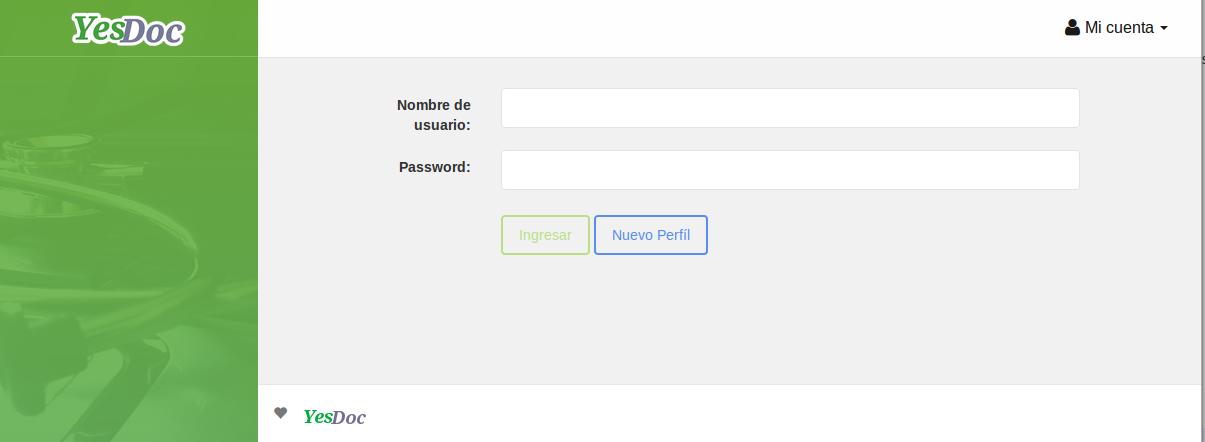
\includegraphics[width=.8\textwidth]{img/manual_de_usuario/iniciar_sesion}
 	\caption{Pantalla de iniciar sesión}
 	\label{mu-iniciar_sesion}
 \end{figure}

\textbf{Posibles errores}
\begin{itemize}
	\item \textbf{Lo sentimos, existe un problema con la conexión al servidor.}
	
	En caso de ver este mensaje de error, verifique que su dispositivo se encuentre conectado a una red de internet o datos 3g (o superior) e intente nuevamente. Si sigue apareciendo el mismo error, comuníquese con su proveedor de internet para asegurarse que la conexión funciones correctamente.
	
	Si a pesar de no haber problemas con su conexión de internet, continua obteniendo el mismo mensaje, envíe un correo electrónico a nuestro equipo de soporte yesdoc@gmail.or
	
	\item \textbf{Usuario o contraseña inválida}
	
	Para ingresar a \textbf{\textit{YesDoc}} debe poseer un usuario válido y conocer su respectiva contraseña. Si no cumple alguna o ambas de estas condiciones debe presionar en el botón de \textbf{\textit{``Nuevo Perfil''}}. \textbf{Figura \ref{mu-us_invalido_ingresar_caracteres}}
	
	\item \textbf{Debe ingresar un usuario}
	
	Los campos de formulario son obligatorios y es necesario que ingrese los valores solicitados para que el botón de ingresar se habilite.\textbf{Figura \ref{mu-us_invalido_ingresar_caracteres}}
	\item \textbf{Debe ingresar un identificador}
	
	Los campos de formulario son obligatorios y es necesario que ingrese los valores solicitados para que el botón de ingresar se habilite.	\textbf{Figura \ref{mu-us_invalido_ingresar_caracteres}}
\end{itemize}
 \begin{figure}
 	\centering
 	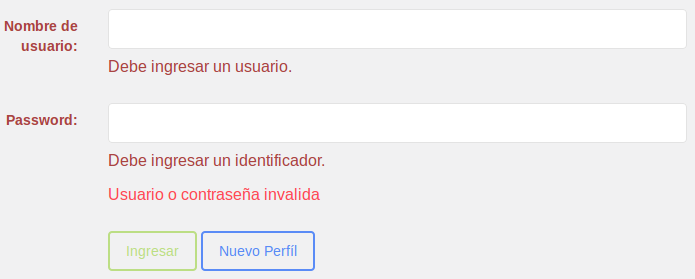
\includegraphics[width=.8\textwidth]{img/manual_de_usuario/us_invalido_ingresar_caracteres}
 	\caption{Pantalla de iniciar sesión}
 	\label{mu-us_invalido_ingresar_caracteres}
 \end{figure}

\subsection{Crear Nuevo Perfil}
Para crear un nuevo perfil debe presionar en el botón \textbf{\textit{``Nuevo perfil''}}, y una vez que el sistema lo direcciona al formulario de creación de usuario, debe llenarlo con todos sus datos.

El Nombre de usuario y el correo electrónico son valores únicos que no debe tener ninguna otra persona, por este motivo es necesario que elija un nombre de usuario que no exista. 

Una vez cargado por completo el formulario debe presionar en enviar y será redireccionado a la página de inicio de sesión para que inicie sesión.

\textbf{Posibles errores}
\begin{itemize}
	\item \textbf{Debe ingresar su nombre de usuario}
	Los campos de formulario son obligatorios y es necesario que ingrese los valores solicitados para que el botón de ingresar se habilite.	\textbf{Figura \ref{mu-nuevo_usuario}}
	\item \textbf{Ya existe una cuenta asociada con este nombre de usuario}	
	Para que ud pueda ser identificado en \textbf{\textit{YesDoc}}, se le solicita que su nombre de usuario sea único.	
	\item \textbf{Debe ingresar su nombre}
	Los campos de formulario son obligatorios y es necesario que ingrese los valores solicitados para que el botón de ingresar se habilite.	\textbf{Figura \ref{mu-nuevo_usuario}}
	\item \textbf{Debe ingresar su apellido}
	Los campos de formulario son obligatorios y es necesario que ingrese los valores solicitados para que el botón de ingresar se habilite.	\textbf{Figura \ref{mu-nuevo_usuario}}
	\item \textbf{Debe ingresar un fecha de nacimiento valida}
Este error ocurre cuando la fecha ingresada es posterior a la actual, para solucionarlo debe ingresar un valor igual o anterior al actual
	\item \textbf{Debe seleccionar un género}
		Los campos de formulario son obligatorios y es necesario que ingrese los valores solicitados para que el botón de ingresar se habilite.	\textbf{Figura \ref{mu-nuevo_usuario}}. Los géneros posibles a ingresar son \textbf{Femenino} y \textbf{Masculino}
	\item \textbf{Debe ingresar un correo electrónico}
		Para que ud pueda ser identificado en \textbf{\textit{YesDoc}} y garantizarle seguridad, se le solicita que ingrese un correo electrónico que no haya sido utilizado con anterioridad, de este modo podremos asociar su información personal a su cuenta única.
	\item \textbf{Debe ingresar un correo electrónico válido}	
	El formato de correo electrónico  es \textbf{\textit{cualquiercosa``@''otracosa.algo}} necesariamente tiene que ingresar un correo electrónico compuesto del simbolo \textbf{\textit{``@''}}
	\item \textbf{Ya existe una cuenta asociada con esta dirección de correo}			
			Para que ud pueda ser identificado en \textbf{\textit{YesDoc}} y garantizarle seguridad, se le solicita que ingrese un correo electrónico que no haya sido utilizado con anterioridad, de este modo podremos asociar su información personal a su cuenta única.
	\item \textbf{Debe ingresar una contraseña}	
		Los campos de formulario son obligatorios y es necesario que ingrese los valores solicitados para que el botón de ingresar se habilite.	\textbf{Figura \ref{mu-nuevo_usuario}}. Para garantizar la seguridad total de su información le solicitamos la contraseña con la cual se encriptarán todos sus datos.
\end{itemize}
 \begin{figure}
 	\centering
 	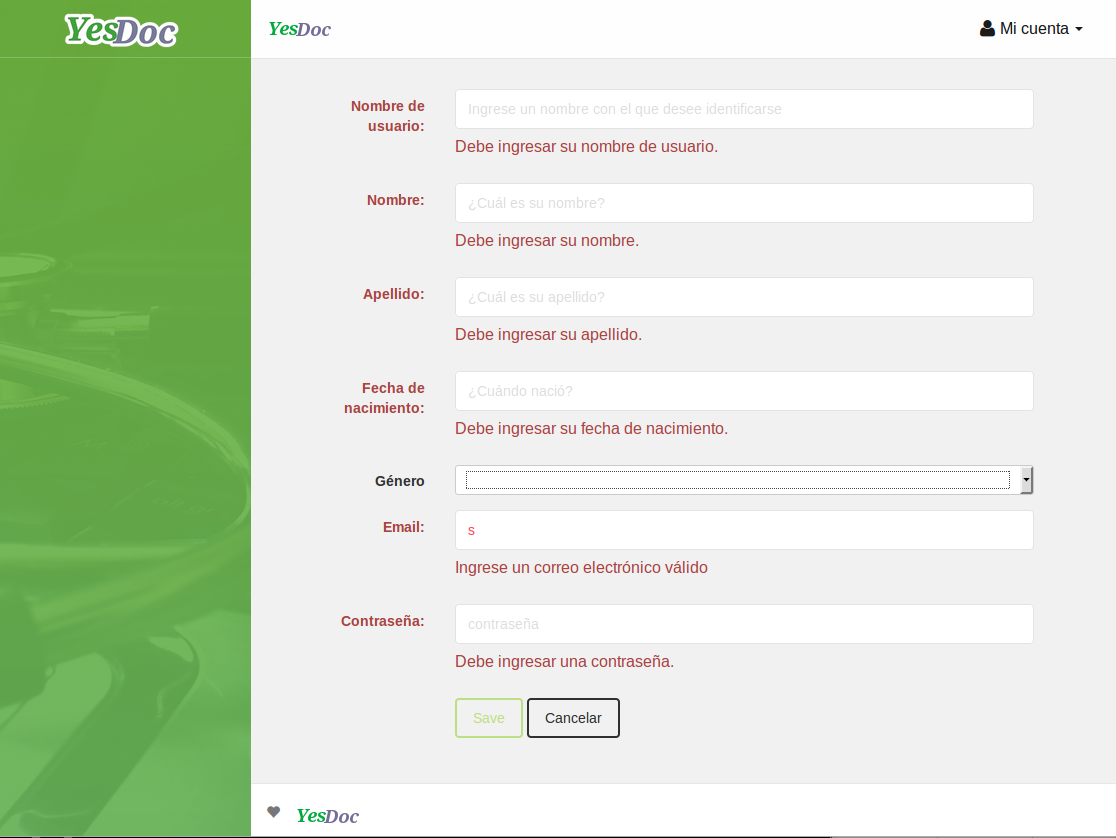
\includegraphics[width=.8\textwidth]{img/manual_de_usuario/nuevo_usuario}
 	\caption{Posibles errores al crear nuevo usuario}
 	\label{mu-nuevo_usuario}
 \end{figure}


\subsection{Información Personal} 
Una vez que ha iniciado se le mostrará la vista de su información personal donde puede ver sus datos y los grupos que tiene asociado a los que les puede compartir la información que ud mas desee \textbf{[Figura \ref{mu-informacion_personal}]}. 

A esta sección se accede haciendo click en su nombre de usuario que se encuentra arriba a la derecha \textbf{Figura \ref{mu-opcion_usuario} }, una vez presionado el botón se desplegarán distintas opciones como \textbf{\textit{``información personal''``Configurar Almacenamiento''``Cerrar sesión''}}, ud debe seleccionar en \textbf{\textit{``Información Personal''}}
  \begin{figure}
  	\centering
  	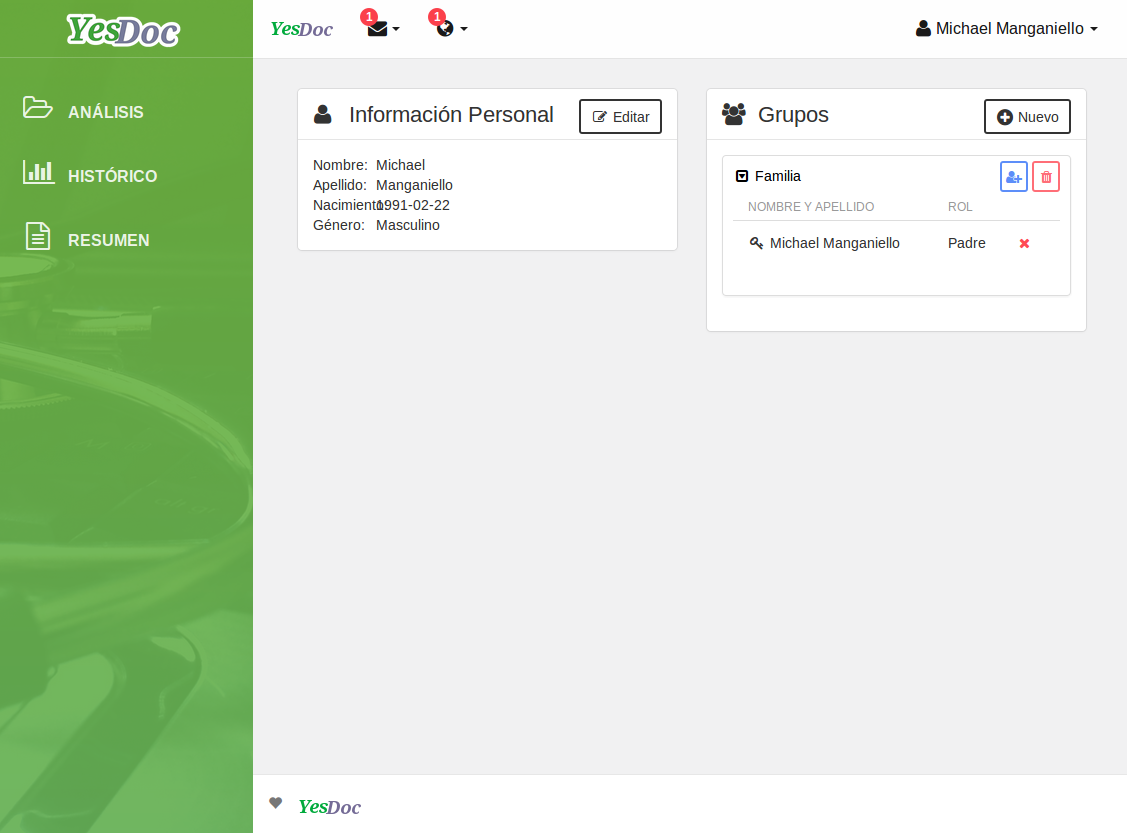
\includegraphics[width=.8\textwidth]{img/manual_de_usuario/informacion_personal}
  	\caption{Perfil de la información personal del usuario}
  	\label{mu-informacion_personal}
  \end{figure}
    \begin{figure}
    	\centering
    	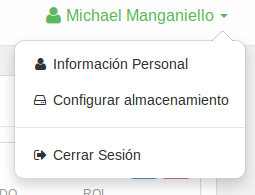
\includegraphics[width=.5\textwidth]{img/manual_de_usuario/opcion_usuario}
    	\caption{Diferentes opciones de la cuenta de usuario                                                                                                                                                                                                                                                                                                                                                                                                                                                                                                  }
    	\label{mu-opcion_usuario}
    \end{figure}
    

\subsection{Grupos}    
En la sección de información personal ud puede ver dos tarjetas     importantes, una de ellas, la ubicada a la derecha, con el título \textbf{\textit{`Grupos''}} se refiere al conjunto de personas, cada uno con permisos asociados, que como conjunto permite facilitar la compartición de análisis médicos, ya que al darle permisos a un grupo sobre un análisis, se ahorra el proceso de brindar acceso a cada una de las personas por separado. Además, si se añaden o se quitan miembros del grupo, los permisos existentes de los análisis antiguos se modifican dinámicamente.

Cabe aclarar que si no posee  grupos la tarjeta se vería como la imagen de la \textbf{Figura \ref{mu-sin_grupos}}
     \begin{figure}
     	\centering
     	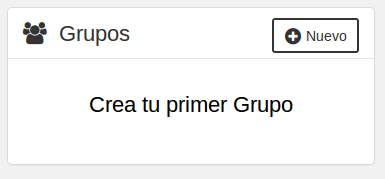
\includegraphics[width=.5\textwidth]{img/manual_de_usuario/sin_grupos}
     	\caption{Tarjeta de grupos, sin grupos cargados}
     	\label{mu-sin_grupos}
     \end{figure}   
\subsubsection{Crear Grupo}
Para crear un grupo debe dirigirse al botón \textbf{``Nuevo''}ubicado arriba a la derecha de la tarjeta de grupos, una vez seleccionado le aparecerá un formulario \textbf{Figura \ref{mu-crear_grupo}} que le permitirá cargar la información necesaria.

\begin{itemize}
	\item \textbf{Nombre:} Nombre del grupo con el que va a identificar al conjunto de personas que va a asociar a tal grupo.
	\item  \textbf{descripción } una breve descripción para recordar con que fin fue  creado el grupo.
	\item \textbf{Tipo de membresía: } existen diversos tipos que caracterizan de manera general los permisos que van a tener los integrantes del grupo.
	\item \textbf{Permisos propios:} Permite aclarar los permisos específicos que los integrantes van a tener sobre un análisis en particular.
\end{itemize}
    \begin{figure}
    	\centering
    	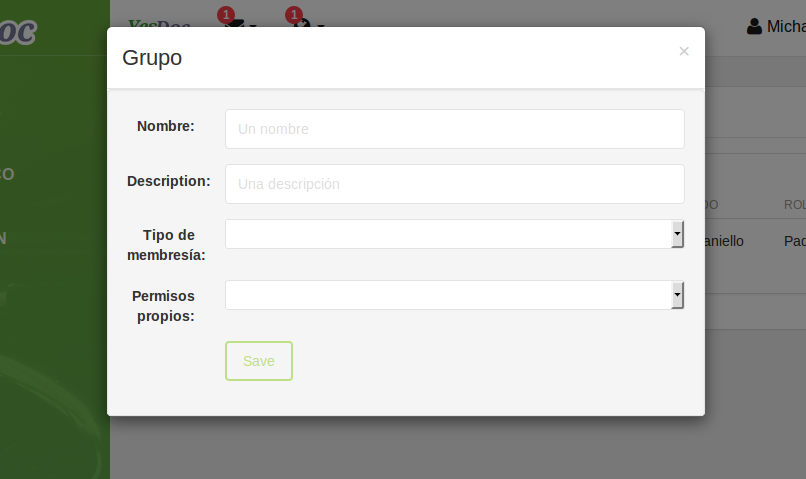
\includegraphics[width=.8\textwidth]{img/manual_de_usuario/crear_grupo}
    	\caption{Formulario para creación de grupo}
    	\label{mu-crear_grupo}
    \end{figure}



\textbf{Posibles errores}

\textbf{Figura \ref{mu-crear_grupo_errores}}
\begin{itemize}
	\item \textbf{Debe ingresar un nombre:} Este aviso se presenta cuando no se ha ingresado el nombre solicitado en el formulario, cabe aclarar que si no se cargan todos los datos obligatorios el botón de enviar no se activa.
	\item \textbf{Seleccione un tipo de membresía: } Este aviso se presenta cuando no se ha seleccionado el tipo de membresía solicitado en el formulario, cabe aclarar que si no se cargan todos los datos obligatorios el botón de enviar no se activa.
	\item \textbf{Permisos Propios:} Este aviso se presenta cuando no se ha seleccionado un tipo de  permisos propios, cabe aclarar que si no se cargan todos los datos obligatorios el botón de enviar no se activa.
\end{itemize}

    \begin{figure}
    	\centering
    	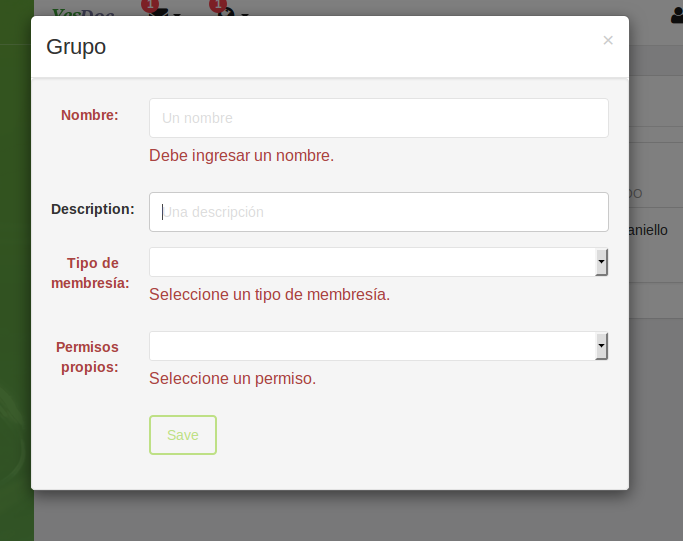
\includegraphics[width=.8\textwidth]{img/manual_de_usuario/crear_grupo_errores}
    	\caption{posibles errores al crear un grupo}
    	\label{mu-crear_grupo_errores}
    \end{figure}


\subsubsection{Cargar miembro al grupo}

Una vez creado el grupo, dentro de la tarjeta de grupos que se ve en la \textbf{Figura \ref{mu-sin_grupos}} aparecerá em nombre del grupo acompañado de dos iconos más, uno para añadir miembros y otro para borrar el grupo. Si desea cargar miembros al grupo debe seleccionar el icono de un muñeco con un símbolo más. Una vez hecho esto, se desplegará un formulario \textbf{Figura \ref{mu-anadir_miembro}} el cual debe completarse con el nombre del miembro, este miembro debe ser un usuario existente, el tipo de membresía y los permisos correspondientes que se le desea dar.
    \begin{figure}
    	\centering
    	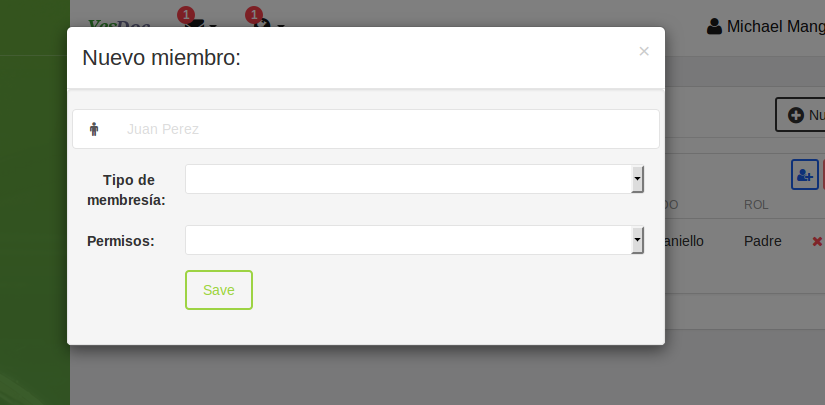
\includegraphics[width=.8\textwidth]{img/manual_de_usuario/aniadir_miembro}
    	\caption{Vista para añadir miembro}
    	\label{mu-anadir_miembro}
    \end{figure}
Una vez realizada la carga el nuevo miembro se listara dento del tipo de grupo, para verlo debe presionar en el icono de despliegue del grupo.

\subsubsection{Eliminar miembro}
Para eliminar un miembro de un grupo en particular primero debe seleccionar el grupo al que pertenece el miembro, al desplegarse el grupo se listarán los miembros, a la derecha de cada miembro hay una cruz que al presionarla elimina el miembro del grupo.

Tenga cuidado en no eliminarse a ud mismo ya que quedaría fuera del grupo.

\subsubsection{Eliminar Grupo}

Para eliminar el grupo debe presionar sobre el icono con forma de papelera que se encuentra al lado del grupo que desea eliminar.
    \begin{figure}
    	\centering
    	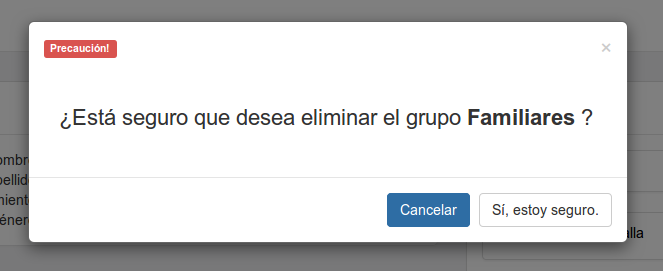
\includegraphics[width=.8\textwidth]{img/manual_de_usuario/eliminar_grupo}
    	\caption{Eliminar grupo}
    	\label{mu-eliminar_grupo}
    \end{figure}
    
    
    
    
    
\subsection{Resumen de mediciones}    
Para dirigirse a la sección de resumen de mediciones debe seleccionar en la sección \textbf{``Resumen''} ubicado en la botonera vertical derecha de color verde, si ud está viendo la aplicación en un celular, la botonera se encontrará del lado izquierdo.

Una vez presionado en resumen podrá ver la pantalla de la \textbf{Figura\ref{mu-resumen_medicion}}
 

    \begin{figure}
    	\centering
    	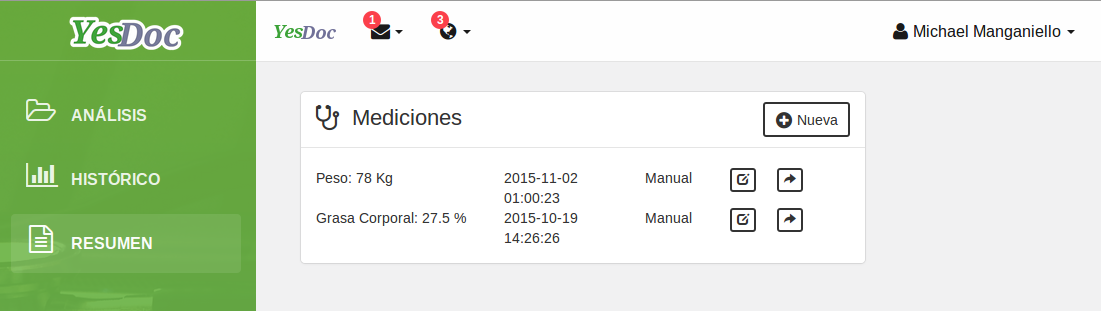
\includegraphics[width=.8\textwidth]{img/manual_de_usuario/resumen_medicion}
    	\caption{Perfil de la mediciones -resumen-}
    	\label{mu-resumen_medicion}
    \end{figure}


\subsubsection{Cargar Nueva Medición}
Para cargar una nueva medición, debe ir a la sección de resumen de mediciones y luego en la tarjeta referida a mediciones debe seleccionar el icono que se encuentra arriba a al derecha que dice \textbf{``Nueva''}, una vez seleccionado le aparece un formulario que debe completar con los datos solicitados.

El botón de enviar dl formulario se encuentra deshabilitado hasta que ingrese todos los valores:
\textbf{tipo, valor, unidad, fuente, fecha}


\textbf{Posibles Errores}
\begin{itemize}
	\item \textbf{Debe seleccionar un tipo de medición} Este mensaje aparece si no se ha seleccionado un tipo de medición en particular, una vez seleccionado va a ir cambiando los valores posibles a elegir según que tipo de medición seleccione.
	\item \textbf{Alerta! El valor ingresado esta fuera de nuestros parámetros normales. Si está seguro que es correcto ignore este mensaje} Este mensaje le avisa que el valor ingresado no es un valor normal, usted puede cargar la medición que mas desee pero debe tener cuidado ya que esos valores influyen en la toma de decisiones del doctor.
	\item \textbf{Debe ingresar un valor númerico.} Este aviso indica que se ha ingresado un valor con letras.
	\item \textbf{Seleccione una fuente de medición.} Debe seleccionar la fuente para poder brindar mejores resultados y conclusiones, si ud no selecciona una fuente el botón de enviar no se deshabilitará
	\item \textbf{Seleccione un tipo de medición.} Debe seleccionar el tipo de medición para poder brindar mejores resultados y conclusiones, si ud no selecciona una fuente el botón de enviar no se deshabilitará
\end{itemize}


\subsection{Listar Análisis}
Para dirigirse a la sección de resumen de mediciones debe seleccionar en la sección \textbf{``Análisis''} ubicado en la botonera vertical derecha de color verde, si ud está viendo la aplicación en un celular, la botonera se encontrará del lado izquierdo.

Una vez presionado en resumen podrá ver la pantalla de la \textbf{Figura\ref{mu-listar_analisis}}


\begin{figure}
	\centering
	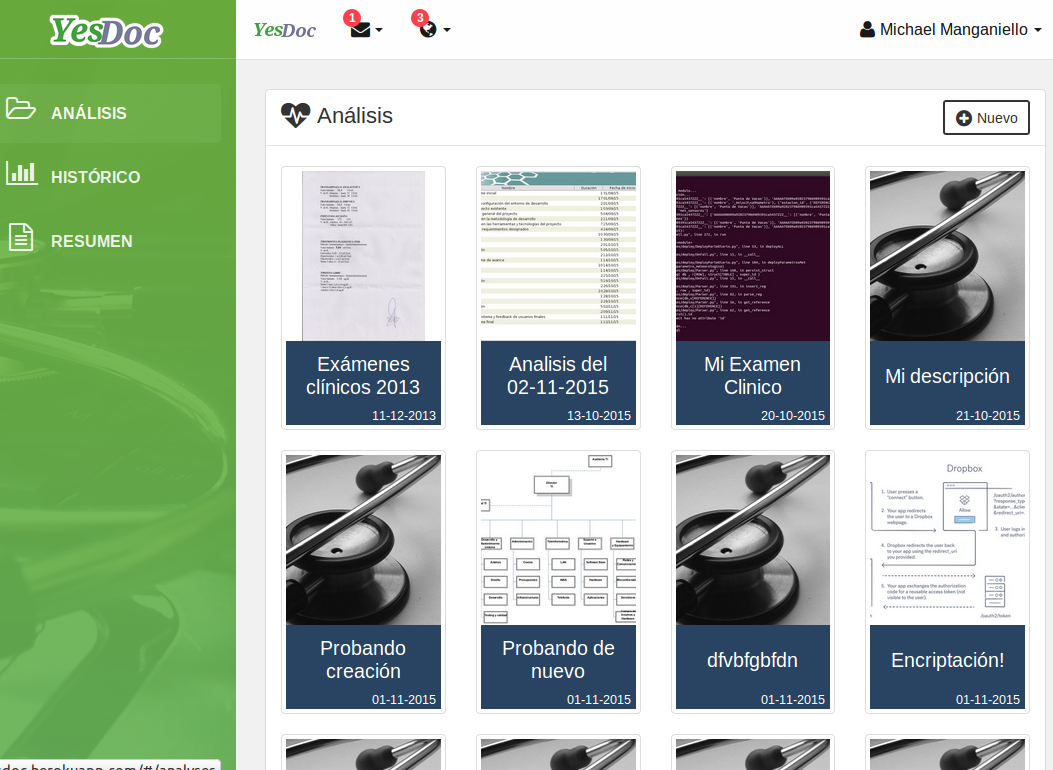
\includegraphics[width=.8\textwidth]{img/manual_de_usuario/listar_analisis}
	\caption{Lista de análisis cargadas por el usuario}
	\label{mu-listar_analisis}
\end{figure}
 
 
 En esta pantalla se muestran todos los análisis con una imagen de portada que trata de describir el contenido del mismo, si el análisis no posee imágenes se muestra una imagen por defecto. Además al pie de cada imagen del análisis se muestra el título y la fecha del mismo.
 
 \subsubsection{Cargar Análisis}
 \subsubsection{Mostrar Análisis particular}
Para ver un análisis en particular, debe seleccionar el análisis, de la lista de análisis, que ud desea ver. Esa acción lo llevará a una interfaz como la de la \textbf{Figura \ref{mu-analisis_particular}}
\begin{figure}
	\centering
	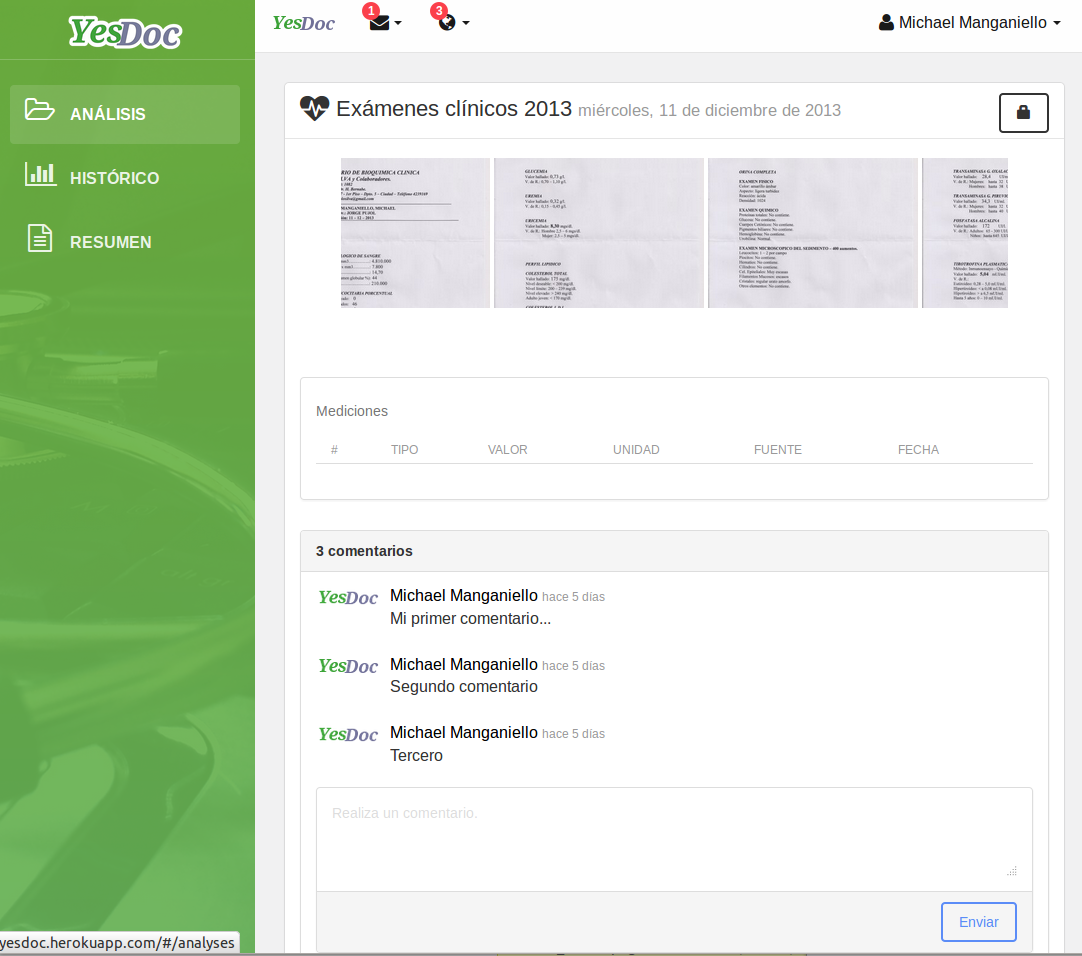
\includegraphics[width=.8\textwidth]{img/manual_de_usuario/analisis_particular}
	\caption{Vista del análisis particular}
	\label{mu-analisis_particular}
\end{figure}
 \subsubsection{Realizar comentarios sobre análisis}
 Para realizar un comentario sobre un análisis, debe seleccionar el análisis y una vez en el, al final del detalle, donde se muestran imágenes y mediciones, se encuentra una sección que le permite ingresar el comentario .

\subsubsection{Compartir análisis}
Para compartir un análisis primero debe seleccionar el análisis y una vez que haya ingresado, debe posicionar en el icono del candado ubicado arriba a la derecha de la tarjeta del análisis y presionarlo. 

Luego de esto  se le mostrará una pantalla donde le permite seleccionar el usuario y el permiso correspondiente \textbf{[Figura \ref{mu-configurar_permiso}]}.

\begin{figure}
	\centering
	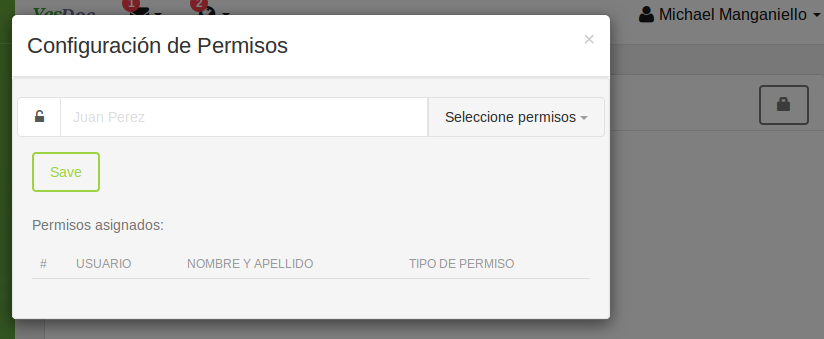
\includegraphics[width=.8\textwidth]{img/manual_de_usuario/configurar_permiso}
	\caption{Configurar los permisos y compartir análisis}
	\label{mu-configurar_permiso}
\end{figure}



\subsection{Historial de mediciones}
Para dirigirse a la sección de historial análisis donde debe seleccionar en la sección \textbf{``Histórico''} ubicado en la botonera vertical derecha de color verde, si ud está viendo la aplicación en un celular, la botonera se encontrará del lado izquierdo.

Una vez presionado en resumen podrá ver la pantalla de la \textbf{Figura\ref{mu-historico}}, donde se ven las gráficas y las tablas correspondientes a las mediciones de un mismo tipo.

El tipo de medición que se muestra, se selecciona presionando el botón que se encuentra arriba a la derecha de la ficha titulada \textbf{Gráficas}.

\begin{figure}
	\centering
	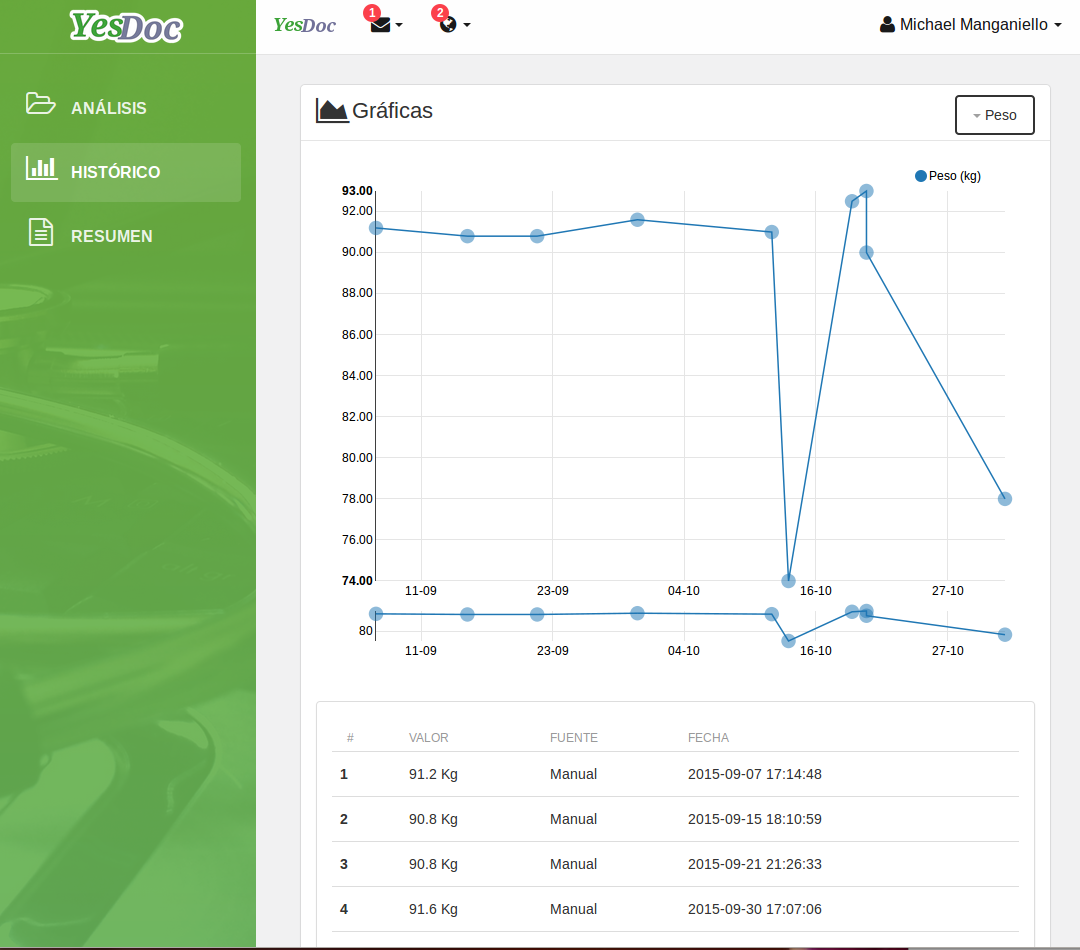
\includegraphics[width=.8\textwidth]{img/manual_de_usuario/historico}
	\caption{Historial de mediciones representado en gráficas y tablas}
	\label{mu-historico}
\end{figure}

\subsection{Notificaciones}
En la botonera horizontal se encuentra un icono de un mundo con un globo que indica la cantidad de notificaciones no leídas. Si Ud selecciona en el icono le listará las últimas 10 notificaciones \textbf{[Figura \ref{mu-notificaciones_vista_previa}}, correspondiente a compartición de análisis, comentarios en análisis y creación de grupos. 
\begin{figure}
	\centering
	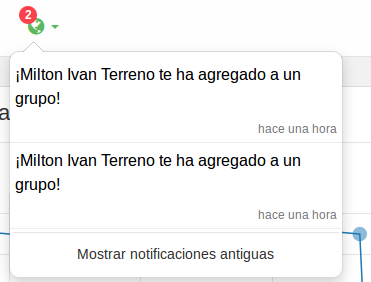
\includegraphics[width=.8\textwidth]{img/manual_de_usuario/notificaciones_vista_previa}
	\caption{Historial de mediciones representado en gráficas y tablas}
	\label{mu-notificaciones_vista_previa}
\end{figure}
Se le permite seleccionar la notificación en particular provocando que se lo redirija a lugar donde se encuentra el evento, ya sea el análisis donde se realizó o el comentario, o la sección de grupos a donde ha sido añadido.

Si selecciona en \textbf{``Mostrar notificaciones antiguas''} se le mostrará todas las notificaciones que le fueron avisadas con la posibilidad de seleccionar cualquiera de ella.

\begin{figure}
	\centering
	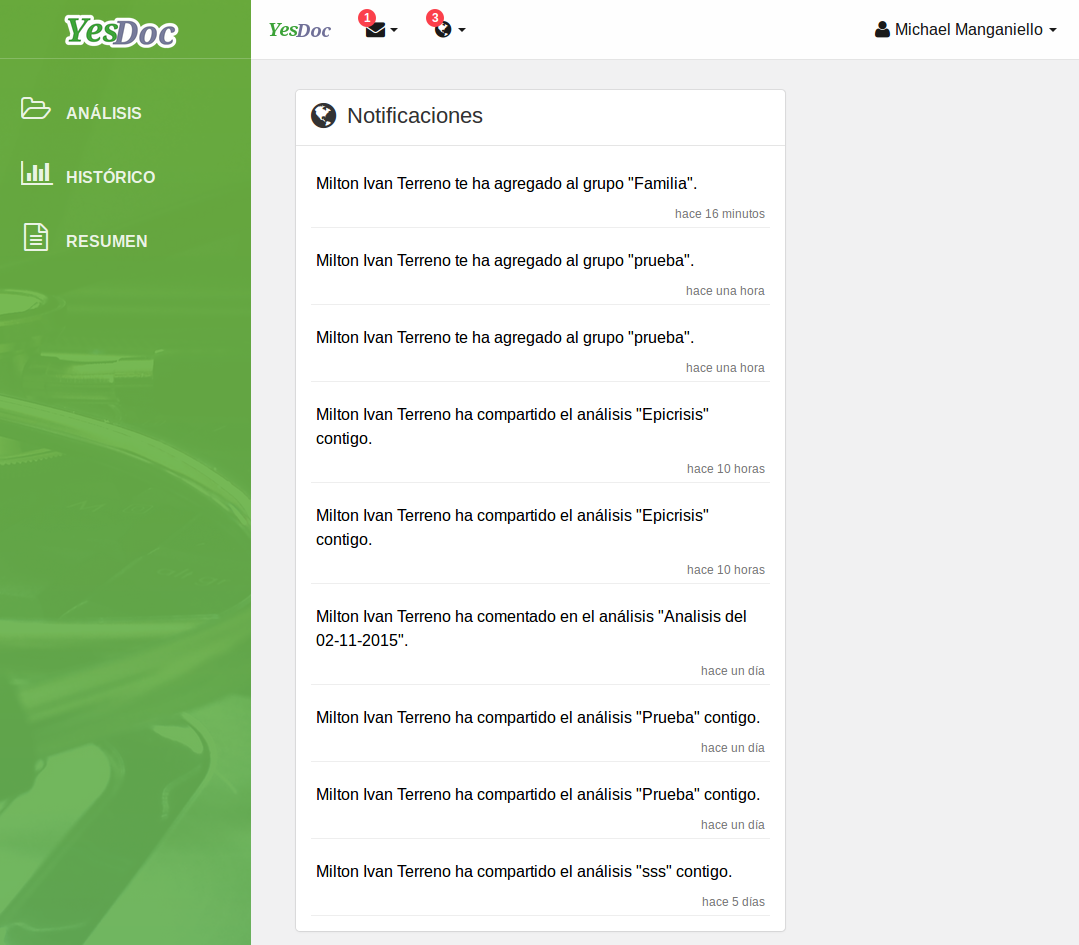
\includegraphics[width=.8\textwidth]{img/manual_de_usuario/lista_notificaciones}
	\caption{Listado de todas las notificaciones}
	\label{mu-lista_notificaciones}
\end{figure}

\subsection{Configurar almacenamiento}
Debe dirigirse a su nombre de usuario ubicado arriba a la derecha \textbf{Figura \ref{mu-opcion_usuario}} y presionar en \textbf{Configurar almacenamiento}. Configurar almacenamiento le permite decidir donde guardar su datos. Una vez presionado el resultado se muestra en la \textbf{Figura}

\begin{figure}
	\centering
	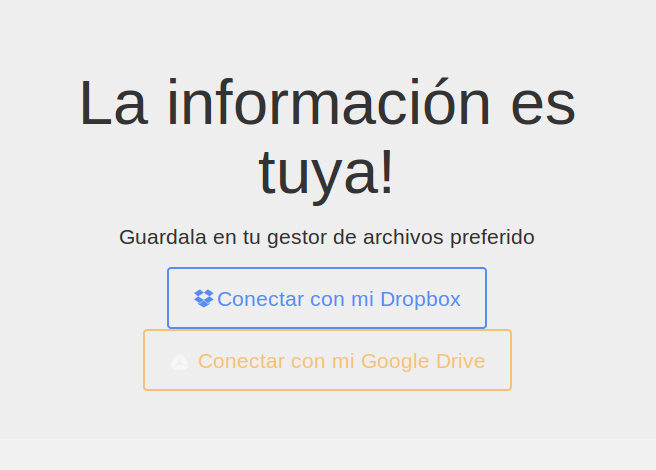
\includegraphics[width=.8\textwidth]{img/manual_de_usuario/configurar_almacenamiento}
	\caption{Opciones de configuración}
	\label{mu-configurar_almacenamiento}
\end{figure}
\begin{figure}
	\centering
	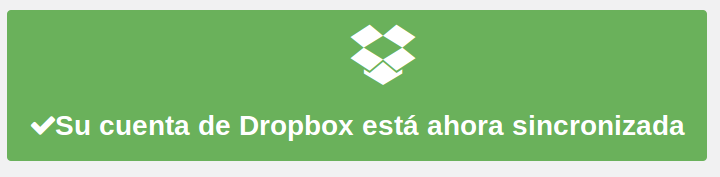
\includegraphics[width=.8\textwidth]{img/manual_de_usuario/cuenta_sincronizada}
	\caption{Mensaje de sincronización}
	\label{mu-cuenta_sincronizada}
\end{figure}
\subsection{Cerrar sesión}
Debe dirigirse a su nombre de usuario ubicado arriba a la derecha \textbf{Figura \ref{mu-opcion_usuario}} y presionar en \textbf{Cerrar Sesión}




% Este comando se utiliza para indicar hasta dónde se cargan las secciones que van en el índice del manual.
% Por lo tanto, siempre debe permanecer al final del archivo.
\stopcontents
